\chapter{Results and discussion}
The implemented parser and planner makes a correct parsing and planning for four different example inputs, which are shown in Table \ref{tab:exampleinput} and Table \ref{tab:exampleinput2}. As seen in the second example sentence, it also handles ambiguous sentences, i.e. handles multiple parse trees. The first parse tree both refers to move all blocks in the world and an non-existing block, which is the reason for the error message ''no such block''. All the plannings below assumes that holding is null and the inital world shown in Figure \ref{fig:initworld}.\\
\begin{figure}[h!]
\centering
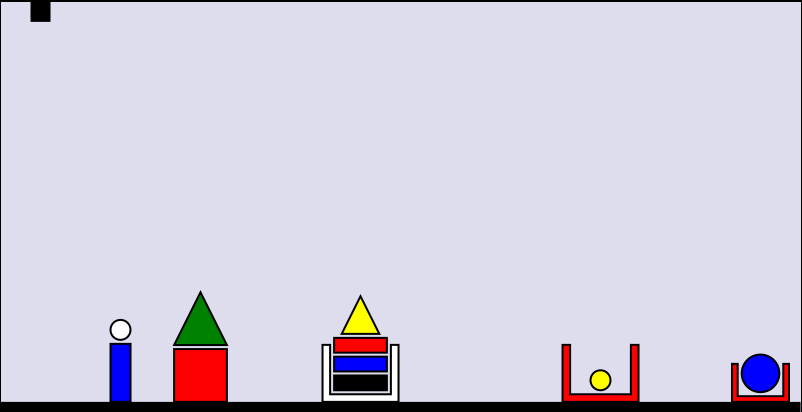
\includegraphics[scale = 0.4]{fig/1.png}
\caption{The initial world\\ $[[],[a,b],[c,d], [], [e,f,g,h,i],[],[],[j,k], [], [l,m]]$}
\label{fig:initworld}
\end{figure}\\
\begin{table}[h!]
\centering
\begin{tabular}{| p{6cm} | p {5.8cm} | p{1.8cm} | }
\hline
\textbf{Input} & \textbf{Parse trees (concrete syntax)} & \textbf{Planning} \\ \hline
Put the blue block that is to the left of a pyramid in a medium-sized box. & ( move ( the ( thatis ( block \_ \_ blue ) ( leftof ( any ( block pyramid \_ \_ ) ) ) ) ) ( inside ( any ( block box medium \_ ) ) ) ) & 
pick 1\linebreak
drop 8\linebreak
pick 9\linebreak
drop 6\linebreak
pick 1\linebreak
drop 9
\linebreak\\ \hline
Move all wide blocks inside a box on top of the red square. & ( move ( all ( block \_ wide \_ ) ) ( inside ( any ( thatis ( block box \_ \_ ) ( ontop ( the ( block square \_ red ) ) ) ) ) ) )  \newline \newline \newline
( move ( all ( thatis ( block \_ wide \_ ) ( inside ( any ( block box \_ \_ ) ) ) ) ) ( ontop ( the ( block square \_ red ) ) ) ) & "no such block" \newline \newline \newline \newline \newline
pick 4\linebreak
drop 8\linebreak
pick 2\linebreak
drop 6\linebreak
pick 4\linebreak
drop 2\linebreak
pick 4\linebreak
drop 2\linebreak
pick 4\linebreak
drop 2\linebreak\\ \hline
\end{tabular}
\caption{Result of the given example sentences in the initial world}
\label{tab:exampleinput}
\end{table}\\
\begin{table}[h!]
\centering
\begin{tabular}{| p{6cm} | p {5.8cm} | p{1.8cm} | }
\hline
Put the wide blue block under the black rectangle. & ( move ( the ( block \_ wide blue ) ) ( under ( the ( block rectangle \_ black ) ) ) ) & 
pick 4\linebreak
drop 8\linebreak
pick 4\linebreak
drop 6\linebreak
pick 4\linebreak
drop 6\linebreak
pick 4\linebreak
drop 6\linebreak \\ \hline
Move all wide rectangles into a red box. & ( move ( all ( block rectangle wide \_ ) ) ( inside ( any ( block box \_ red ) ) ) ) & 
pick 4\linebreak
drop 8\linebreak
pick 7\linebreak
drop 6\linebreak
pick 4\linebreak
drop 7\linebreak
pick 4\linebreak
drop 7\linebreak
pick 4\linebreak
drop 7\linebreak\\ \hline
\end{tabular}
\caption{Result of the given example sentences in the initial world}
\label{tab:exampleinput2}
\end{table}\\
All the examples in Table \ref{tab:exampleinput} and Table \ref{tab:exampleinput2} refers to a $Move$ action. An example of how the planning is done is shown in Figure \ref{fig:moveex}. The implemented parser and planner also handles the actions $Take$ and $Put$. Examples of these are shown below in Table \ref{tab:put_take}. The $Put$ action assumes that there is a block in holding, in this case the world is the same as above but with holding the red square.\\\\
\begin{table}[h!]
\centering
\begin{tabular}{| p{6cm} | p {5.8cm} | p{1.8cm} | }
\hline
\textbf{Input} & \textbf{Parse trees (concrete syntax)} & \textbf{Planning} \\ \hline
Take the red square! & 	(take (the (block square \_ red ) ) ) & 
pick 2\linebreak
drop 8\linebreak
pick 2\linebreak\\ \hline
Put it on the floor & ( put ( ontop floor) ) & drop 6\linebreak \\ \hline
\end{tabular}
\caption{Result of actions $Take$ and $Put$ (when holding the block from the $Take$ action}
\label{tab:put_take}
\end{table}\\\\
\begin{figure}
\centering
\begin{subfigure}{.5\textwidth}
  \centering
  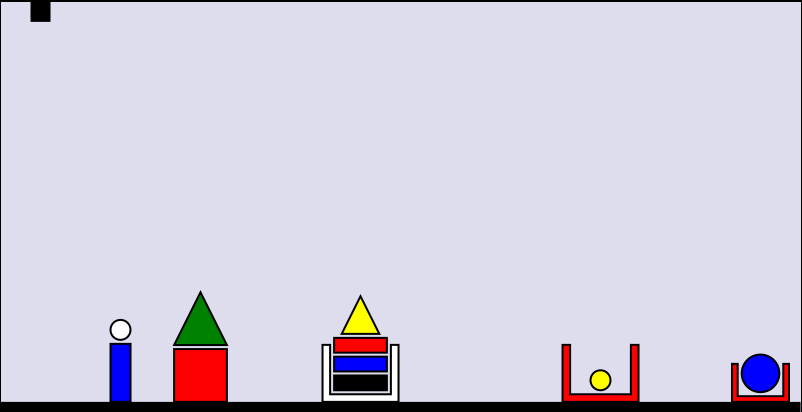
\includegraphics[width=.7\linewidth]{fig/1.png}
  \caption{Inital state}
  \label{fig:1}
\end{subfigure}%
\begin{subfigure}{.5\textwidth}
  \centering
  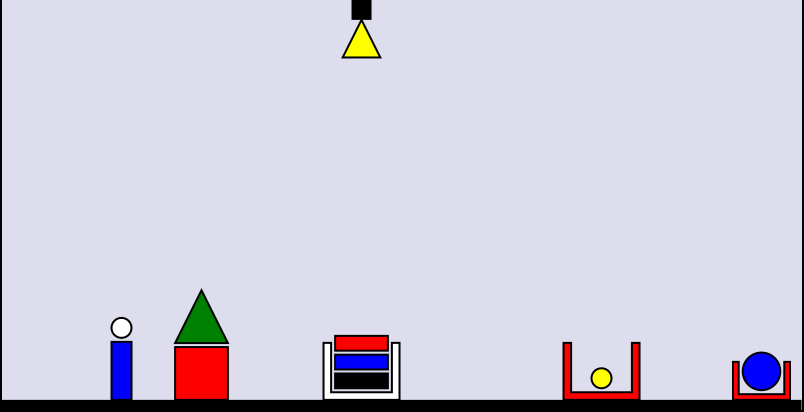
\includegraphics[width=.7\linewidth]{fig/2.png}
  \caption{Take the yellow pyramid}
  \label{fig:2}
\end{subfigure}
\begin{subfigure}{.5\textwidth}
  \centering
  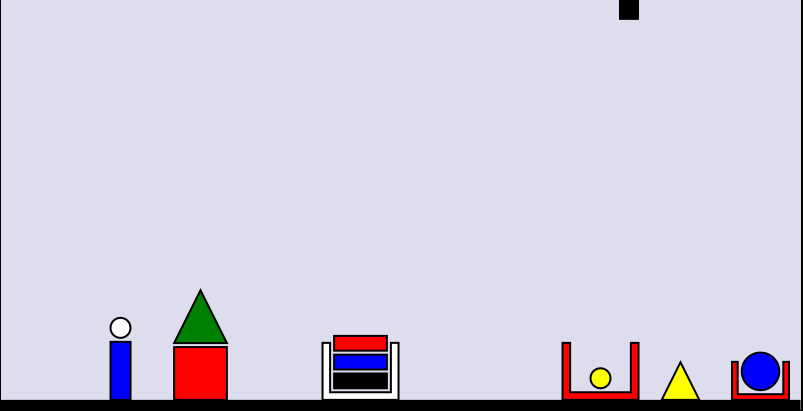
\includegraphics[width=.7\linewidth]{fig/3.png}
  \caption{Drop the yellow pyramid}
  \label{fig:3}
\end{subfigure}%
\begin{subfigure}{.5\textwidth}
  \centering
  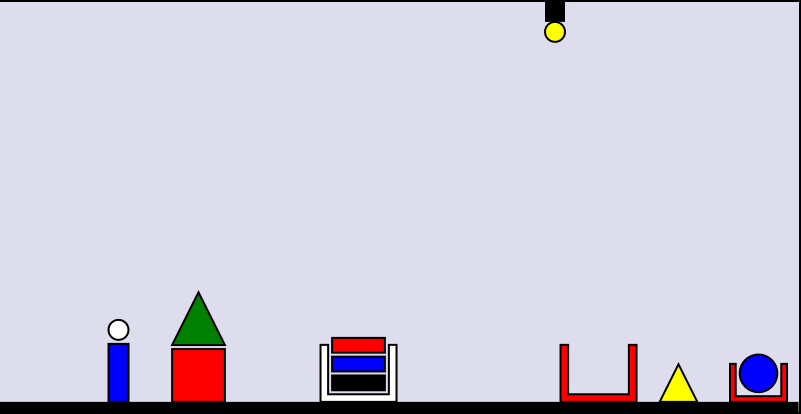
\includegraphics[width=.7\linewidth]{fig/4.png}
  \caption{Take the yellow ball}
  \label{fig:4}
\end{subfigure}
\begin{subfigure}{.5\textwidth}
  \centering
  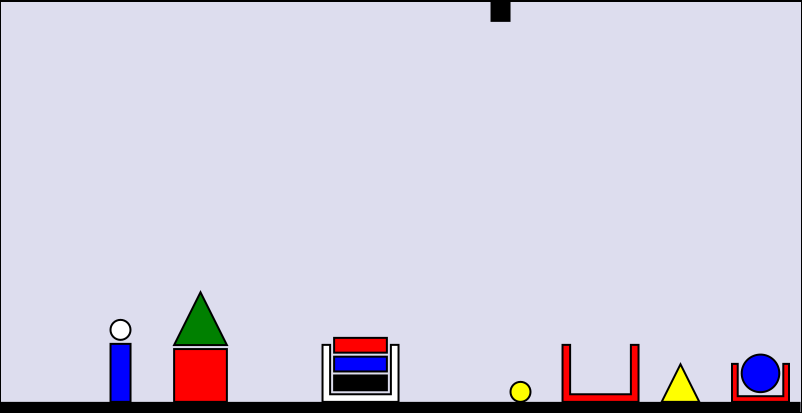
\includegraphics[width=.7\linewidth]{fig/5.png}
  \caption{Drop the yellow ball}
  \label{fig:5}
\end{subfigure}%
\begin{subfigure}{.5\textwidth}
  \centering
  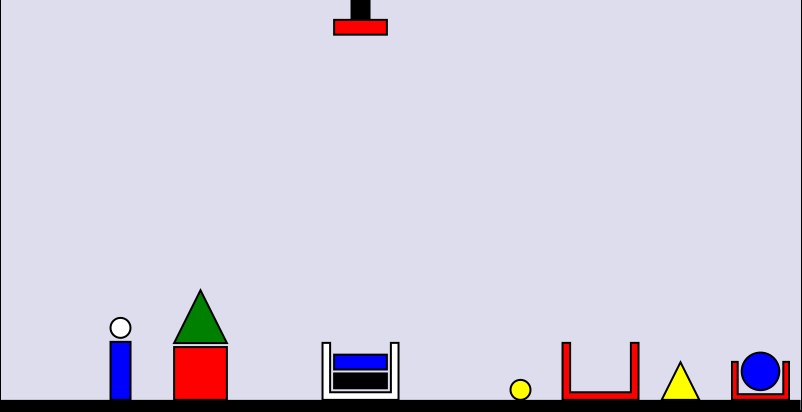
\includegraphics[width=.7\linewidth]{fig/6.png}
  \caption{Take the red rectangle}
  \label{fig:6}
\end{subfigure}
\begin{subfigure}{.5\textwidth}
  \centering
  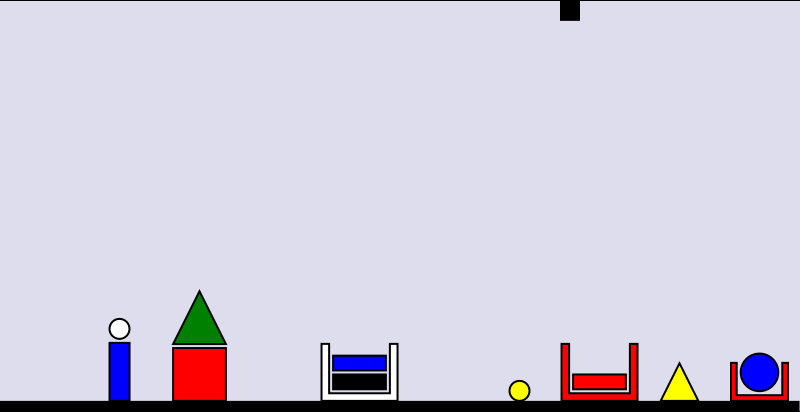
\includegraphics[width=.7\linewidth]{fig/7.png}
  \caption{Drop the red rectangle}
  \label{fig:7}
\end{subfigure}%
\begin{subfigure}{.5\textwidth}
  \centering
  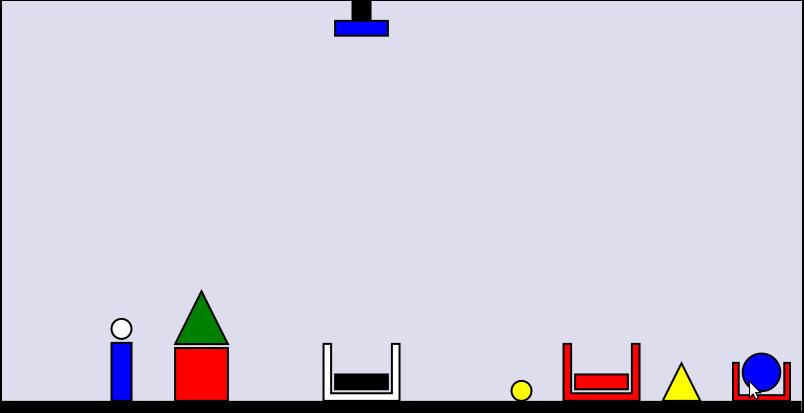
\includegraphics[width=.7\linewidth]{fig/8.png}
  \caption{Take the blue wide rectangle}
  \label{fig:8}
\end{subfigure}
\begin{subfigure}{.5\textwidth}
  \centering
  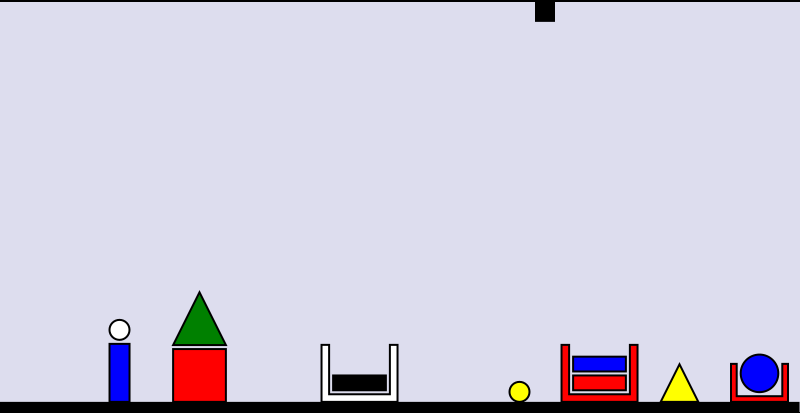
\includegraphics[width=.7\linewidth]{fig/9.png}
  \caption{Drop the blue wide rectangle}
  \label{fig:9}
\end{subfigure}%
\begin{subfigure}{.5\textwidth}
  \centering
  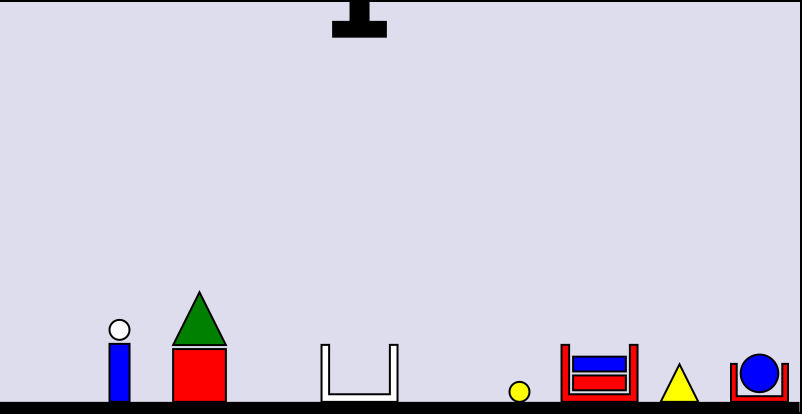
\includegraphics[width=.7\linewidth]{fig/10.png}
  \caption{Take the black rectangle}
  \label{fig:10}
\end{subfigure}
\begin{subfigure}{.5\textwidth}
  \centering
  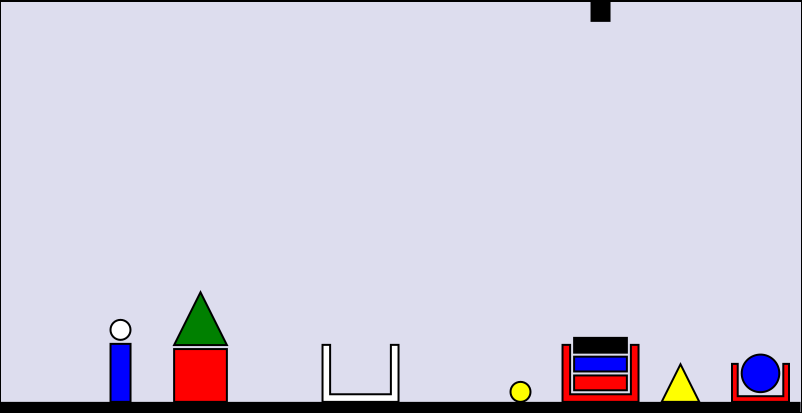
\includegraphics[width=.7\linewidth]{fig/11.png}
  \caption{Drop the black rectangle}
  \label{fig:11}
\end{subfigure}
\caption{The figure shows how the blocks are moved for the action: ''Move all wide rectangles into a red 
box.''}
\label{fig:moveex}
\end{figure}\\
Of course there is several sentences which is not handled by the parser and the planner. An example of a such sentence is "Move all blocks inside a box on top of the red square." which results in a timeout due to our translation of the command. The parser returns a list of all blocks that is inside of a box, to be moved. This is impossible to perform in the initial world since there is two boxes with a ball inside and balls can never be put on each other. Then the planner will not find a solution, which results in a timeout.\\\\
The planner does not print what it does, such as ''I move the topmost block from stack X to stack Y''. The planning is just shown visually and in form of pick and drop instructions. \\\\\\\\
The planner will not try to optimize the time it takes to perform the instructions, i.e. it might not drop blocks at the closest available stack. This does not affect the number of instructions, which we try to optimize. Also, the planner will not try to restore blocks to their inital positions if it has move them to reach another block or position. The planner does not guarantee that we move the right block, i.e. if block A should be moved to the left of block B the planner might move block B to the right of block A instead. 
\\\\
If the sentence is ambiguous, the parser will return multiple parse tree but the planner will only choose the first valid parse tree. In the example sentence 2, the first parse tree is treated as invalid.
\section{Discussion}
A big problem when handling natural language is that there is many ways of read things which easily makes a sentence ambiguous. We also noticed that it was hard to cover all cases that could occur in the parser and depending on which input we got it was possible to pattern match on power sets of possible inputs, which the code increase rapidly. \\\\
Another difficulty in the beginning was that the syntax tree that was given from the parser was a concrete syntax tree and we wanted an abstract syntax tree to be able to pattern match on the different parts. This was solved when we found a library which could convert between GF grammar as concrete and abstract syntax. \\\\
We also choosed to implement a planning algorithm by graph traversal, by implementing A*. Another possibility would been to use for example First-Order Logic instead. 
\\\\
We did a lot of tweaking with the heuristic function and notice how instable it was. There might be cases that we miss and there is a lot of ways of making a heuristic function.
